%%%%%% better tables
% install in R: reporttools and stargazer

\documentclass[11pt]{article}

\usepackage{longtable} % for tables

\usepackage{adjustbox} 


\title{My first replicable Paper}
\author{
        MyFirstName MyLastName\\
        Evans School of Public Policy and Governance\\
        University of Washington\\
        Seattle, WA 98115, \underline{United States}\\
        \texttt{greatguy@uw.edu}
}
\date{\today}


\usepackage{Sweave}
\begin{document}
\Sconcordance{concordance:PaperInR_5.tex:PaperInR_5.Rnw:%
1 21 1 1 0 30 1 1 7 8 1 1 5 4 1 1 7 29 0 1 2 5 1 1 9 4 1 2 2 14 1 1 7 %
14 0 1 2 4 1 1 8 4 1 2 2 16 1 1 5 3 1 2 2 12 1 1 5 4 1 2 2 10 1}


\maketitle 

\begin{abstract}
This is an example on how to make a reproducible paper. We are using R from Rstudio, creating an RSweave document. This is a nice start to create a nice paper and get an A+. The next sections will show the steps taken.
\end{abstract}


\section{Introduction}\label{intro}

This is my intro to my great paper, I will explain the cool things I can do with my new `computational thinking' powers combined with some Latex. This is my intro to my great paper, I will explain the cool things I can do with my new `computational thinking' powers combined with some Latex. This is my intro to my great paper, I will explain the cool things I can do with my new `computational thinking' powers combined with some Latex. This is my intro to my great paper, I will explain the cool things I can do with my new `computational thinking' powers combined with some Latex.


This is my nice intro to my great paper, 
I will explain the cool things 
I can do with my new `computational thinking' 
powers
combined with some Latex.


\section{Exploring Data}\label{explo}


Sections may use a label\footnote{In fact, you can have a label wherever you think a future reference to that content might be needed.}. This label is needed for referencing. For example the next section has label \emph{datas}, so you can reference it by writing: As we see in section \ref{catexplo}.






\subsection{Exploring Categorical Data}\label{catexplo}

Here, I continue doing this nice work, I hope you like it and read it. It has been a very hard work.Here, I continue doing this nice work, I hope you like it and read it. It has been a very hard work.Here, I continue doing this nice work, I hope you like it and read it. It has been a very hard work.Here, I continue doing this nice work, I hope you like it and read it. It has been a very hard work.Here, I continue doing this nice work, I hope you like it and read it. It has been a very hard work.Here, I continue doing this nice work, I hope you like it and read it. It has been a very hard work.

You can see the statistics of categorical variables in Table \ref{catexplore_table}.

%%%%%% LOADING LIBRARIES


%%%%%% stats for categorical columns
% table for categorical variables
% USING "results=tex" 

% latex table generated in R 3.6.2 by xtable 1.8-4 package
% Fri Feb  7 11:53:05 2020
\begingroup\normalsize
\begin{longtable}{llrrr}
\caption{Freq Table} \\ 
 \textbf{Variable} & \textbf{Levels} & $\mathbf{n}$ & $\mathbf{\%}$ & $\mathbf{\sum \%}$ \\ 
  \hline
Region & Africa & 55 & 27.1 & 27.1 \\ 
   & Asia & 45 & 22.2 & 49.3 \\ 
   & Eurasia & 6 & 3.0 & 52.2 \\ 
   & Europe & 45 & 22.2 & 74.4 \\ 
   & NAmerica & 26 & 12.8 & 87.2 \\ 
   & Oceania & 14 & 6.9 & 94.1 \\ 
   & SAmerica & 12 & 5.9 & 100.0 \\ 
   \hline
 & all & 203 & 100.0 &  \\ 
   \hline
\hline
ONIpolitical & nd & 2 & 2.6 & 2.6 \\ 
   & per & 8 & 10.5 & 13.2 \\ 
   & sub & 4 & 5.3 & 18.4 \\ 
   & sel & 21 & 27.6 & 46.0 \\ 
   & ne & 41 & 54.0 & 100.0 \\ 
   \hline
 & all & 76 & 100.0 &  \\ 
   \hline
\hline
\hline
\label{catexplore_table}
\end{longtable}
\endgroup

%%%%%%

You can see this variable plotted in Figure \ref{catexplore_plot}



\begin{figure}[h]
\centering
\begin{adjustbox}{width=7cm,height=5cm}
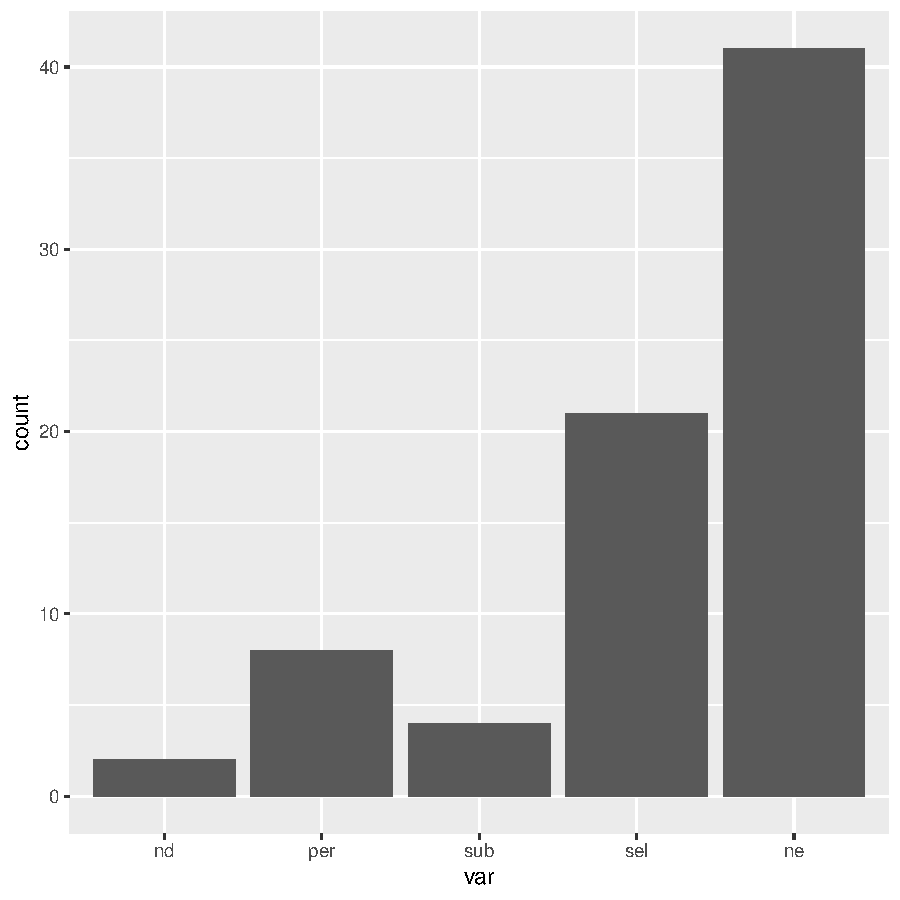
\includegraphics{PaperInR_5-cat_plot}
\end{adjustbox}
\caption{ONI barplot}  %title
\label{catexplore_plot} % for \ref{}
\end{figure}





\subsection{Exploring Numerical Data}\label{numexplo}

Here, I continue doing this nice work, I hope you like it and read it. It has been a very hard work.Here, I continue doing this nice work, I hope you like it and read it. It has been a very hard work.Here, I continue doing this nice work, I hope you like it and read it. It has been a very hard work.Here, I continue doing this nice work, I hope you like it and read it. It has been a very hard work.Here, I continue doing this nice work, I hope you like it and read it. It has been a very hard work.Here, I continue doing this nice work, I hope you like it and read it. It has been a very hard work.Here, I continue doing this nice work, I hope you like it and read it. It has been a very hard work.Here, I continue doing this nice work, I hope you like it and read it. It has been a very hard work.Here, I continue doing this nice work, I hope you like it and read it. It has been a very hard work.

%%%%%% stats for numeric columns

% Table created by stargazer v.5.2.2 by Marek Hlavac, Harvard University. E-mail: hlavac at fas.harvard.edu
% Date and time: Fri, Feb 07, 2020 - 11:53:06
\begin{table}[!htbp] \centering 
  \caption{Stat summary for nummeric vars} 
  \label{numexplore_table} 
\footnotesize 
\begin{tabular}{@{\extracolsep{5pt}}lccccccc} 
\\[-1.8ex]\hline 
\hline \\[-1.8ex] 
Statistic & \multicolumn{1}{c}{Median} & \multicolumn{1}{c}{Mean} & \multicolumn{1}{c}{Min} & \multicolumn{1}{c}{Max} & \multicolumn{1}{c}{Pctl(25)} & \multicolumn{1}{c}{Pctl(75)} & \multicolumn{1}{c}{St. Dev.} \\ 
\hline \\[-1.8ex] 
FHF & 49.00 & 47.24 & 10.00 & 97.00 & 25.25 & 63.00 & 23.72 \\ 
RWB & 28.72 & 32.40 & 6.38 & 84.83 & 23.60 & 38.50 & 16.64 \\ 
\hline \\[-1.8ex] 
\end{tabular} 
\end{table} 

In the Table \ref{numexplore_table}, you realize that the mean of FHF is {\bf47.24}.




\begin{figure}[h]
\centering
\begin{adjustbox}{width=7cm,height=5.5cm,clip,trim=0cm 0.5cm 0cm 0cm} 
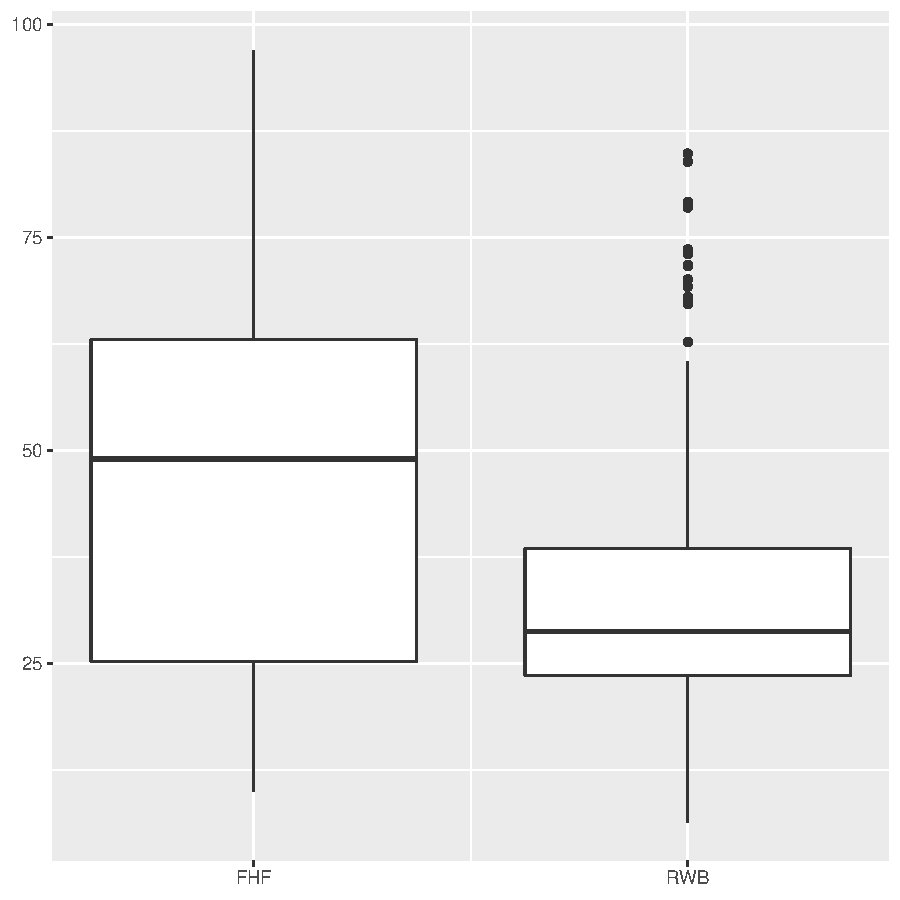
\includegraphics{PaperInR_5-num_plot}
\end{adjustbox}
\caption{boxplots}  
\label{num_plot} 
\end{figure}



Boxplots were introduced by Tuckey (Tukey, John W (1977). Exploratory Data Analysis. Addison-Wesley.)

\section{Looking for Relationships}\label{bivar}


Here, I continue doing this nice work, I hope you like it and read it. It has been a very hard work.Here, I continue doing this nice work, I hope you like it and read it. It has been a very hard work.Here, I continue doing this nice work, I hope you like it and read it. It has been a very hard work.Here, I continue doing this nice work, I hope you like it and read it. It has been a very hard work.Here, I continue doing this nice work, I hope you like it and read it. It has been a very hard work.Here, I continue doing this nice work, I hope you like it and read it. It has been a very hard work.Here, I continue doing this nice work, I hope you like it and read it. It has been a very hard work.Here, I continue doing this nice work, I hope you like it and read it. It has been a very hard work.Here, I continue doing this nice work, I hope you like it and read it. It has been a very hard work.

\subsection{Numerical and  Categorical}\label{binumcat}



\begin{figure}[h]
\centering
\begin{adjustbox}{width=7cm,height=7cm} 
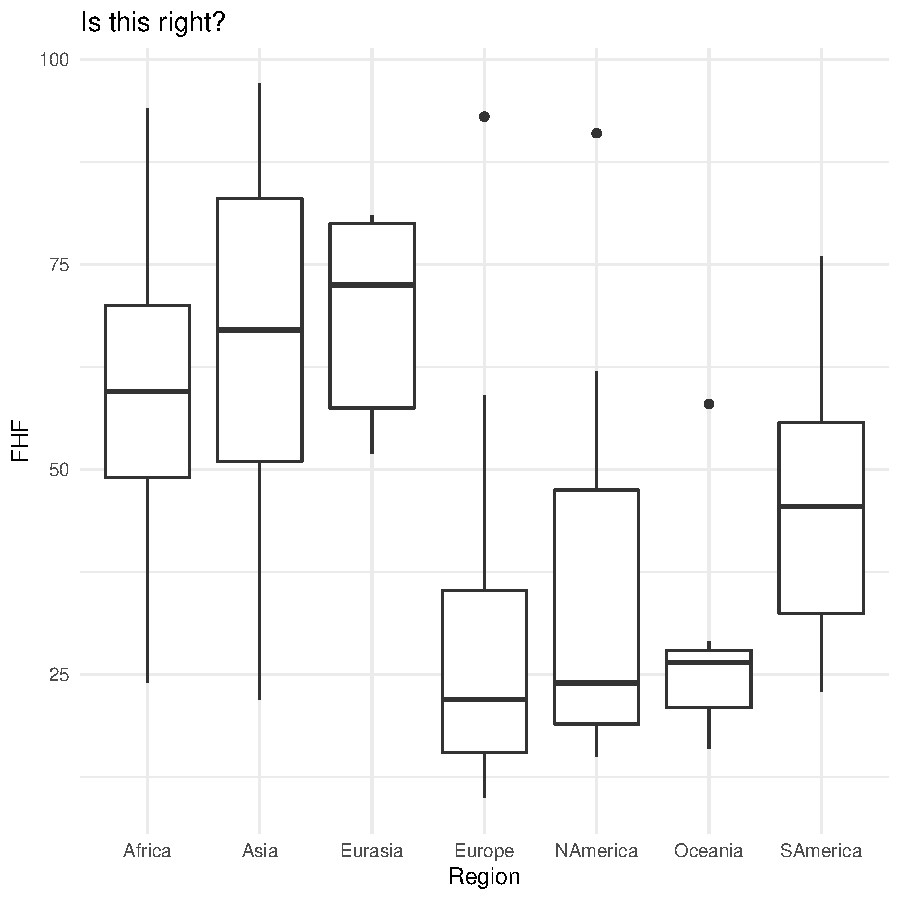
\includegraphics{PaperInR_5-numcat_plot}
\end{adjustbox}
\caption{Boxplots: one numerical by a category.}  
\label{numcat_plot} 
\end{figure}


Here, I continue doing this nice work, I hope you like it and read it. It has been a very hard work.Here, I continue doing this nice work, I hope you like it and read it. It has been a very hard work.Here, I continue doing this nice work, I hope you like it and read it. It has been a very hard work.Here, I continue doing this nice work, I hope you like it and read it. It has been a very hard work.Here, I continue doing this nice work, I hope you like it and read it. It has been a very hard work.Here, I continue doing this nice work, I hope you like it and read it. It has been a very hard work.Here, I continue doing this nice work, I hope you like it and read it. It has been a very hard work.Here, I continue doing this nice work, I hope you like it and read it. It has been a very hard work.Here, I continue doing this nice work, I hope you like it and read it. It has been a very hard work.

\subsection{Numerical and Numerical}\label{binumnum}

Here, I continue doing this nice work, I hope you like it and read it. It has been a very hard work.Here, I continue doing this nice work, I hope you like it and read it. It has been a very hard work.Here, I continue doing this nice work, I hope you like it and read it. It has been a very hard work.Here, I continue doing this nice work, I hope you like it and read it. It has been a very hard work.Here, I continue doing this nice work, I hope you like it and read it. It has been a very hard work.Here, I continue doing this nice work, I hope you like it and read it. It has been a very hard work.Here, I continue doing this nice work, I hope you like it and read it. It has been a very hard work.Here, I continue doing this nice work, I hope you like it and read it. It has been a very hard work.Here, I continue doing this nice work, I hope you like it and read it. It has been a very hard work.




\begin{figure}[h]
\centering
\begin{adjustbox}{width=7cm,height=5.5cm}
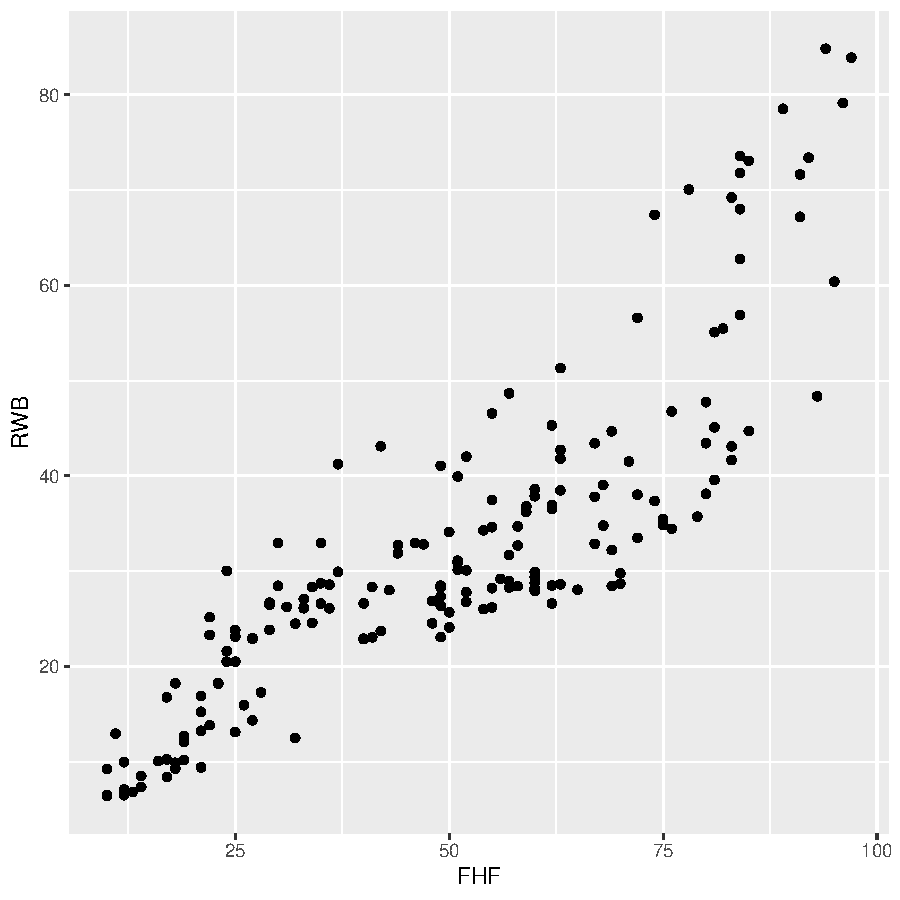
\includegraphics{PaperInR_5-numnum_plot}
\end{adjustbox}
\caption{scatter}  
\label{numnum_plot} 
\end{figure}


The scatter plot is thought to be invented by  John Frederick W. Herschel according to this link: https://qz.com/1235712/the-origins-of-the-scatter-plot-data-visualizations-greatest-invention/



\end{document}
